\documentclass{beamer}
\usepackage{graphicx}
\usepackage{listings} % Syntax highlighing
\usepackage{fancyvrb} % Inline verbatim
\usepackage{hyperref} % Hyperlinks
\hypersetup{pdfpagemode=FullScreen}
\usepackage{tikz}
\usepackage{attachfile}

\usetheme{Boadilla}
\title{More Malware Models}
\author{UMBC Malware Data Science}
\date{Week 9: 31 March 2020}

\begin{document}

\begin{frame}
    In prior Labs, you made some models. Let's take a closer look.
\end{frame}

\begin{frame}{Explainability}
    Explainability is an important topic in machine learning. How do you know if your features mean anything or are helping the model? How do you explain to a peer or supervisor why the model classified a file in a certain way?
    \\ ~~ \\
    Some algorithms, such as decision trees, are explainable. There's also a Python module called \texttt{shap} which allows data scientists to explore feature use and importance in their models.
    \\ ~~ \\
    \texttt{xgboost} is a decision tree algorithm which works well with sparse data, and has optimizations for faster calculations than \texttt{sklearn}, including GPU support (CUDA on Nvidia devices).
\end{frame}

\begin{frame}{xgboost}

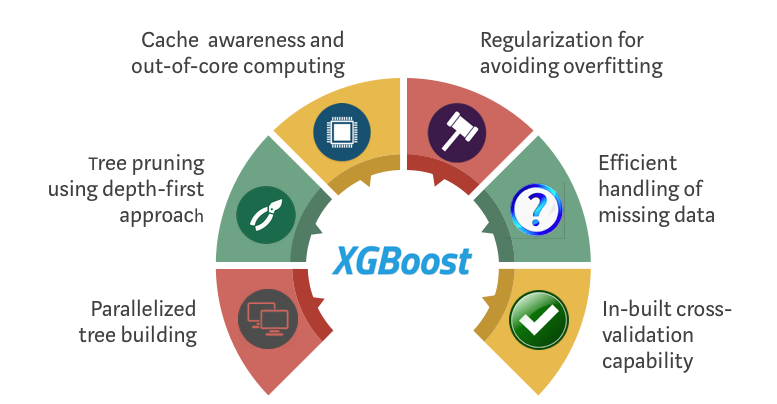
\includegraphics[scale=0.4]{Images/xgboost.png}

Source: \url{https://towardsdatascience.com/https-medium-com-vishalmorde-xgboost-algorithm-long-she-may-rein-edd9f99be63d}
\end{frame}

\begin{frame}{Lab 9}
    For Lab 9, revisit the code \& models from Lab 4, and using \texttt{shap} and \texttt{xgboost}, identify which features are more indicative of maliciousness/goodness, and make a better model. Also note any speed and accuracy improvements.
    \\ ~~ \\
    For next week, read \textit{Kilograms: Very Large N-Grams for Malware Classification} \attachfile{Papers/kilograms.pdf}.
\end{frame}

\end{document}